\documentclass[12pt]{report}

% ---------- PACKAGES ----------
\usepackage[a4paper,margin=1in]{geometry}
\usepackage{graphicx}
\usepackage{tikz}
\usetikzlibrary{arrows.meta, positioning, shapes.geometric}
\usepackage{array}
\usepackage{longtable}
\usepackage{fancyhdr}
\usepackage{titlesec}
\usepackage{hyperref}
\usepackage{xcolor}
\usepackage{enumitem}
\usepackage{capt-of}
\usepackage{float}

% ---------- HEADER/FOOTER ----------
\pagestyle{fancy}
\fancyhf{}
\fancyhead[R]{\textit{UCS503 - Software Engineering}}
\fancyfoot[C]{\thepage}
\renewcommand{\headrulewidth}{0.4pt}
\setlength{\headheight}{15pt}

% ---------- HYPERLINK SETUP ----------
\hypersetup{
    colorlinks=true,
    linkcolor=black,
    urlcolor=blue,
    pdftitle={UCS503 - Collaborative Study Platform}
}

\titleformat{\chapter}[hang]{\normalfont\huge\bfseries}{Chapter \thechapter}{1em}{}

\begin{document}

% =========================================================
% TITLE PAGE
% =========================================================
\begin{titlepage}
    \centering
    \vspace*{1cm}
    {\large UCS503 - Software Engineering}\\[1.5cm]
    {\Huge \bfseries Collaborative Study Platform}\\[0.5cm]
    {\large A Web-Based Academic Resource-Sharing Platform for Students}\\[2cm]

    {\large Submitted by:}\\[0.3cm]
    1024170430 \quad Anirudh\\
    1024170449 \quad Shashvt\\
    1024170441 \quad Lavish\\[0.5cm]
    Group: 5, BE Third Year, CSE\\[2cm]

    {\large Submitted to:}\\[0.3cm]
    Ms Nisha Thakur\\
    Mid-Semester Evaluation\\[2cm]

    \vfill
    Computer Science and Engineering Department\\
    Thapar Institute of Engineering and Technology, Patiala
\end{titlepage}

% =========================================================
% TABLE OF CONTENTS (manually typeset — trimmed after Module 1,
% everything else left exactly as in the original)
% =========================================================
\chapter*{Contents}
\addcontentsline{toc}{chapter}{Contents}

\noindent
\begin{tabular}{@{}ll@{\hspace{0.5em}}r@{}}
\multicolumn{3}{@{}l}{\textbf{Chapter 1 Introduction}\dotfill 3} \\[2pt]
\hspace{1em} 1.1 Background and Context & \dotfill & 3 \\[2pt]
\hspace{2em} 1.1.1 Problem Statement & \dotfill & 3 \\[2pt]
\hspace{1em} 1.2 Project Objectives & \dotfill & 3 \\[6pt]
\multicolumn{3}{@{}l}{\textbf{Chapter 2 Methodology and Design}\dotfill 4} \\[2pt]
\hspace{1em} 2.1 System Architecture & \dotfill & 4 \\[2pt]
\hspace{2em} 2.1.1 High-Level Design & \dotfill & 4 \\[2pt]
\hspace{2em} 2.1.2 Technical Stack & \dotfill & 8 \\[2pt]
\hspace{1em} 2.2 Implementation Details & \dotfill & 8 \\[2pt]
\hspace{2em} 2.2.1 Module 1: Core Functionality & \dotfill & 8 \\
\end{tabular}

\clearpage

% =========================================================
% CHAPTER 1 - INTRODUCTION
% =========================================================
\chapter{Introduction}

\section{Background and Context}
The Collaborative Study Platform is a web-based academic resource-sharing platform designed
primarily for students. Its purpose is to provide students with a centralized place to access and
share academic study material. The platform organizes academic resources according to the
student's academic context, and the major resources available through the platform are Study
Notes, Books, and Previous Year Questions (PYQs). The platform also provides functionality
for uploading study material so that academic resources can be added to the platform.

\subsection{Problem Statement}
Students currently require a centralized place to access and share academic study material
relevant to their specific academic context. The platform addresses this by organizing resources
according to classroom, year/stream, and subject, and by allowing users to both retrieve
existing resources (notes, books, PYQs) and contribute new study material through an upload
facility.

\section{Project Objectives}
\begin{itemize}[leftmargin=*]
    \item To provide a centralized platform where students can access academic Study Notes,
    Books, and Previous Year Questions (PYQs), organized according to their academic
    context (classroom, year/stream, and subject).
    \item To implement a secure user authentication system (registration and login) that
    protects the platform's user-specific functionality.
    \item To allow authenticated students to navigate a dashboard, select their academic context
    (classroom, year/stream, subject), and view or download the corresponding notes,
    books, and PYQs.
    \item To provide functionality for students to upload study material, including entry of
    relevant metadata and selection of a file, so that additional academic resources can be
    added to the platform.
\end{itemize}

% =========================================================
% CHAPTER 2 - METHODOLOGY AND DESIGN
% =========================================================
\chapter{Methodology and Design}

\section{System Architecture}
The platform follows a client-server architecture. The Student/User interacts with the React
Frontend, which communicates with the Go/Gin Backend over REST-style APIs. The backend,
in turn, communicates with PostgreSQL and AWS S3 where required. The user does not
directly communicate with PostgreSQL or AWS S3. Uploaded files are stored in AWS S3,
while the information describing each file (filename, year, subject code, stream, uploader
information, and the AWS S3 reference/key) is stored in PostgreSQL.

\subsection{High-Level Design}
The general system workflow proceeds as follows: user authentication, followed by academic
context selection (classroom, then year/stream, then subject), followed by study resource
access (notes, books, or PYQs) or, optionally, study material upload, after which the user may
continue using the platform or log out. The diagrams below illustrate the actors, workflows, and
interactions that make up this design.

% --- Figure 2.1: UML Use Case Diagram ---
\begin{figure}[H]
    \centering
    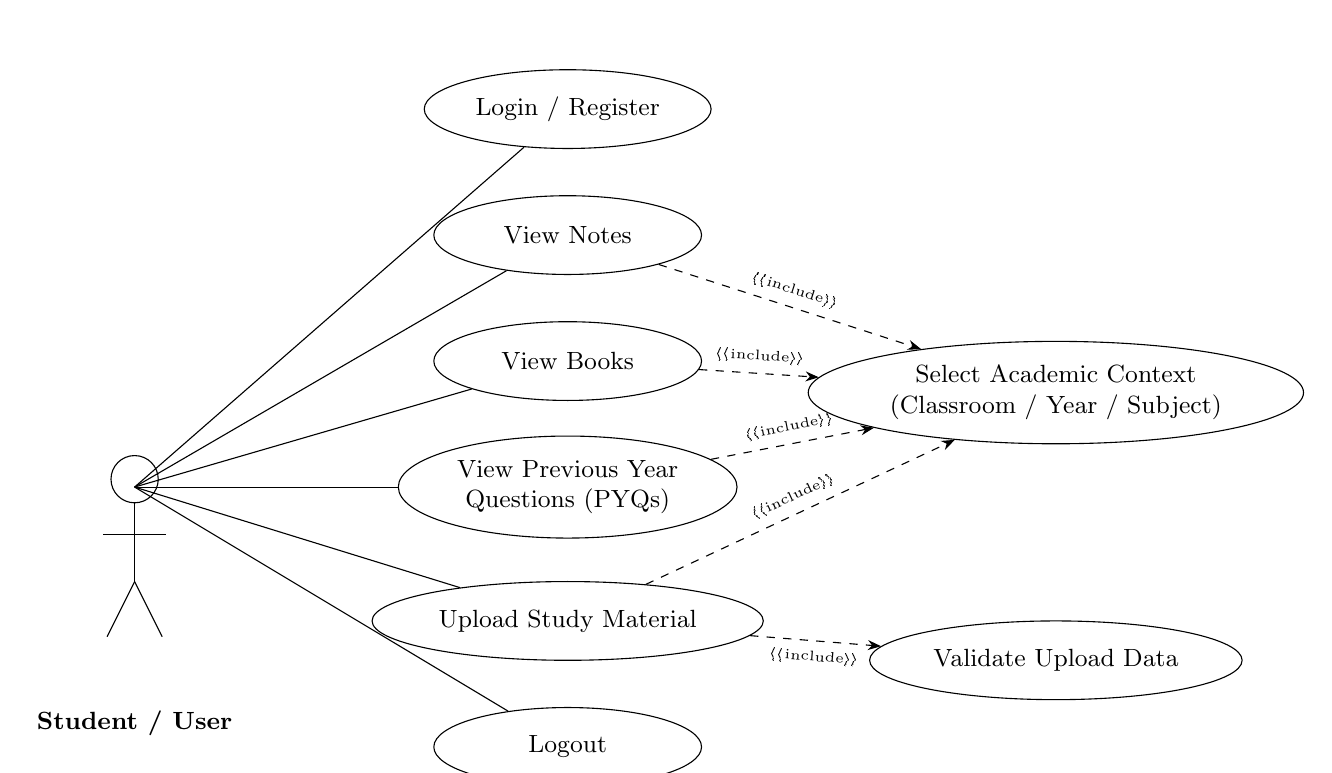
\begin{tikzpicture}[font=\small, >={Stealth[]}]
        % actor (stick figure)
        \begin{scope}[shift={(-5.5,-3.2)}]
            \draw (0,1.1) circle (0.3);
            \draw (0,0.8) -- (0,-0.2);
            \draw (-0.4,0.4) -- (0.4,0.4);
            \draw (0,-0.2) -- (-0.35,-0.9);
            \draw (0,-0.2) -- (0.35,-0.9);
            \node[align=center, yshift=-1.1cm] at (0,-0.9) {\textbf{Student / User}};
        \end{scope}
        \coordinate (actor) at (-5.5,-2.2);

        % use case ellipses (left column) -- generous vertical spacing
        \node[draw, ellipse, minimum width=3.4cm, minimum height=1cm] (login)  at (0, 2.6)  {Login / Register};
        \node[draw, ellipse, minimum width=3.4cm, minimum height=1cm] (notes)  at (0, 1.0)  {View Notes};
        \node[draw, ellipse, minimum width=3.4cm, minimum height=1cm] (books)  at (0,-0.6)  {View Books};
        \node[draw, ellipse, minimum width=3.6cm, minimum height=1cm, align=center] (pyq) at (0,-2.2) {View Previous Year\\Questions (PYQs)};
        \node[draw, ellipse, minimum width=4.0cm, minimum height=1cm] (upload) at (0,-3.9)  {Upload Study Material};
        \node[draw, ellipse, minimum width=3.4cm, minimum height=1cm] (logout) at (0,-5.5)  {Logout};

        % include-target ellipses (right column)
        \node[draw, ellipse, minimum width=4.2cm, minimum height=1.3cm, align=center] (context) at (6.2,-1.0) {Select Academic Context\\(Classroom / Year / Subject)};
        \node[draw, ellipse, minimum width=3.6cm, minimum height=1cm, align=center] (validate) at (6.2,-4.4) {Validate Upload Data};

        % actor associations
        \draw (actor) -- (login);
        \draw (actor) -- (notes);
        \draw (actor) -- (books);
        \draw (actor) -- (pyq);
        \draw (actor) -- (upload);
        \draw (actor) -- (logout);

        % include dependencies
        \draw[dashed,->] (notes)  -- node[above,sloped,font=\tiny]{\textlangle\textlangle include\textrangle\textrangle} (context);
        \draw[dashed,->] (books)  -- node[above,sloped,font=\tiny]{\textlangle\textlangle include\textrangle\textrangle} (context);
        \draw[dashed,->] (pyq)    -- node[above,sloped,font=\tiny]{\textlangle\textlangle include\textrangle\textrangle} (context);
        \draw[dashed,->] (upload) -- node[above,sloped,font=\tiny]{\textlangle\textlangle include\textrangle\textrangle} (context);
        \draw[dashed,->] (upload) -- node[below,sloped,font=\tiny]{\textlangle\textlangle include\textrangle\textrangle} (validate);
    \end{tikzpicture}
    \caption{UML Use Case Diagram -- Collaborative Study Platform}
\end{figure}

The Student/User is the sole actor of the system and can Login/Register, View Notes, View
Books, View Previous Year Questions, Upload Study Material, and Logout. The use cases
View Notes, View Books, View Previous Year Questions, and Upload Study Material each
include the Select Academic Context use case, and Upload Study Material additionally includes
Validate Upload Data.

% --- Table 2.1: Sample Use Case ---
\begin{center}
\begin{longtable}{|p{4cm}|p{9cm}|}
\hline
\multicolumn{2}{|c|}{\textbf{Sample Use Case -- UC-01: User Login}} \\
\hline
\textbf{1. Use Case Title} & User Login \\
\hline
\textbf{2. Abbreviated Title} & Login \\
\hline
\textbf{3. Use Case Id} & UC-01 \\
\hline
\textbf{4. Actors} & Student/User \\
\hline
\textbf{5. Description} & Allows a registered user to authenticate and gain access to the
Collaborative Study Platform using their registered credentials. \\
\hline
\textbf{5.1. Pre Conditions} & User must have a registered account. \\
\hline
\textbf{5.2. Task Sequence} &
1. User opens the login screen.\newline
2. User enters email and password.\newline
3. React Frontend sends the credentials to the Go/Gin Backend for verification.\newline
4. Backend validates credentials against PostgreSQL and returns a session token. \\
\hline
\textbf{5.3. Post Conditions} &
1. User is authenticated and redirected to the Dashboard.\newline
2. Session is stored for subsequent requests. \\
\hline
\textbf{6. Modification History} & Date: 17-Sep-2026 \\
\hline
\textbf{7. Author} & Anirudh \\
\hline
\end{longtable}
\captionof{table}{Sample Use Case Description -- UC-01 User Login}
\end{center}

% --- Figure 2.2: Activity Diagram ---
\begin{figure}[H]
    \centering
    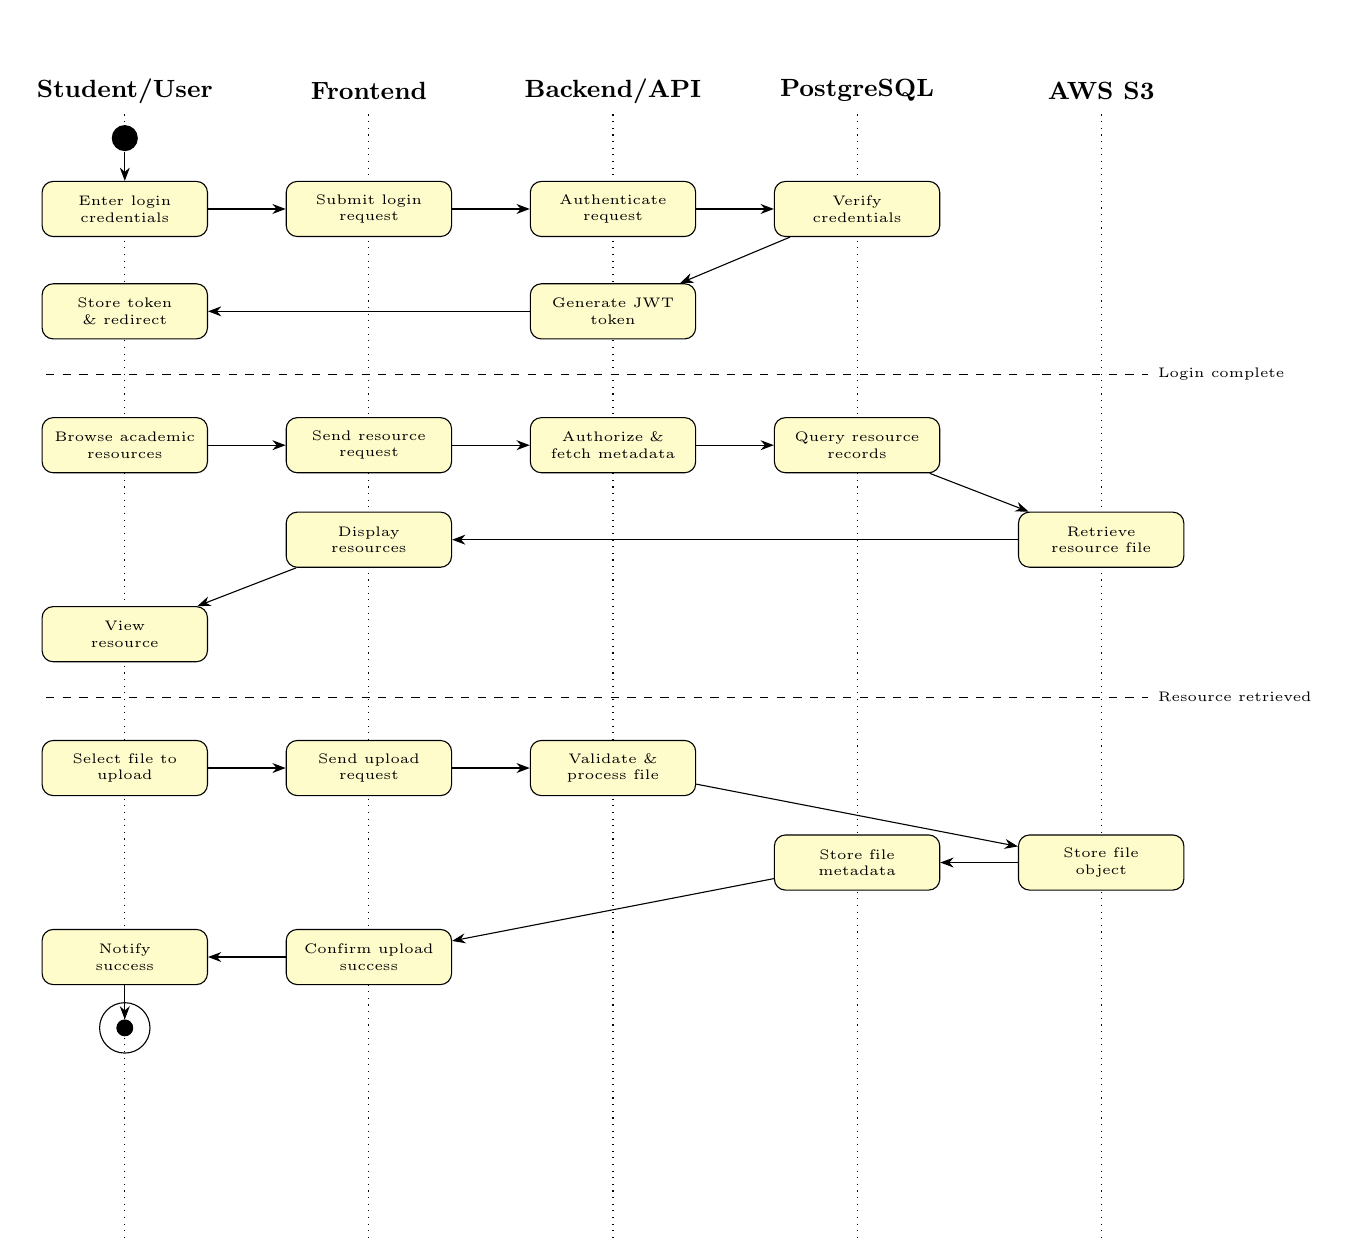
\begin{tikzpicture}[
        font=\tiny,
        act/.style={draw, fill=yellow!20, rounded corners, minimum width=2.1cm, minimum height=0.7cm, align=center},
        >={Stealth[]}
      ]
        % column headers
        \def\cA{0} \def\cB{3.1} \def\cC{6.2} \def\cD{9.3} \def\cE{12.4}
        \node[font=\small\bfseries] at (\cA,0.6) {Student/User};
        \node[font=\small\bfseries] at (\cB,0.6) {Frontend};
        \node[font=\small\bfseries] at (\cC,0.6) {Backend/API};
        \node[font=\small\bfseries] at (\cD,0.6) {PostgreSQL};
        \node[font=\small\bfseries] at (\cE,0.6) {AWS S3};
        \foreach \x in {\cA,\cB,\cC,\cD,\cE}{\draw[dotted] (\x,0.3) -- (\x,-14.2);}

        % start
        \node[circle, fill=black, minimum size=0.25cm] (start) at (\cA,0) {};

        % ---- Phase 1: Login ----
        \node[act] (n1) at (\cA,-0.9) {Enter login\\credentials};
        \node[act] (n2) at (\cB,-0.9) {Submit login\\request};
        \node[act] (n3) at (\cC,-0.9) {Authenticate\\request};
        \node[act] (n4) at (\cD,-0.9) {Verify\\credentials};
        \node[act] (n5) at (\cC,-2.2) {Generate JWT\\token};
        \node[act] (n6) at (\cA,-2.2) {Store token\\\& redirect};

        \draw[->] (start) -- (n1);
        \draw[->] (n1) -- (n2);
        \draw[->] (n2) -- (n3);
        \draw[->] (n3) -- (n4);
        \draw[->] (n4) -- (n5);
        \draw[->] (n5) -- (n6);

        \draw[dashed] (-1,-3.0) -- (13,-3.0) node[right,font=\tiny] {Login complete};

        % ---- Phase 2: Resource access ----
        \node[act] (n7) at (\cA,-3.9)  {Browse academic\\resources};
        \node[act] (n8) at (\cB,-3.9)  {Send resource\\request};
        \node[act] (n9) at (\cC,-3.9)  {Authorize \&\\fetch metadata};
        \node[act] (n10) at (\cD,-3.9) {Query resource\\records};
        \node[act] (n11) at (\cE,-5.1) {Retrieve\\resource file};
        \node[act] (n12) at (\cB,-5.1) {Display\\resources};
        \node[act] (n13) at (\cA,-6.3) {View\\resource};

        \draw[->] (n7) -- (n8);
        \draw[->] (n8) -- (n9);
        \draw[->] (n9) -- (n10);
        \draw[->] (n10) -- (n11);
        \draw[->] (n11) -- (n12);
        \draw[->] (n12) -- (n13);

        \draw[dashed] (-1,-7.1) -- (13,-7.1) node[right,font=\tiny] {Resource retrieved};

        % ---- Phase 3: Upload ----
        \node[act] (n14) at (\cA,-8.0) {Select file to\\upload};
        \node[act] (n15) at (\cB,-8.0) {Send upload\\request};
        \node[act] (n16) at (\cC,-8.0) {Validate \&\\process file};
        \node[act] (n17) at (\cE,-9.2) {Store file\\object};
        \node[act] (n18) at (\cD,-9.2) {Store file\\metadata};
        \node[act] (n19) at (\cB,-10.4) {Confirm upload\\success};
        \node[act] (n20) at (\cA,-10.4) {Notify\\success};

        \draw[->] (n14) -- (n15);
        \draw[->] (n15) -- (n16);
        \draw[->] (n16) -- (n17);
        \draw[->] (n17) -- (n18);
        \draw[->] (n18) -- (n19);
        \draw[->] (n19) -- (n20);

        \node[circle, draw, fill=black, minimum size=0.2cm, inner sep=1pt] (end) at (\cA,-11.3) {};
        \draw[circle, draw] (end) circle (0.32cm);
        \draw[->] (n20) -- (end);
    \end{tikzpicture}
    \caption{Activity Diagram -- Login, Resource Access, and Upload Workflow}
\end{figure}

This activity diagram traces the complete runtime workflow across three phases separated by
synchronization bars: authentication (entering credentials through token storage and redirect),
resource access (browsing academic resources through display of the requested resource), and
study material upload (selecting a file through confirmation and notification of upload success).

% --- Figure 2.3: Swimlane Diagram ---
\begin{figure}[H]
    \centering
    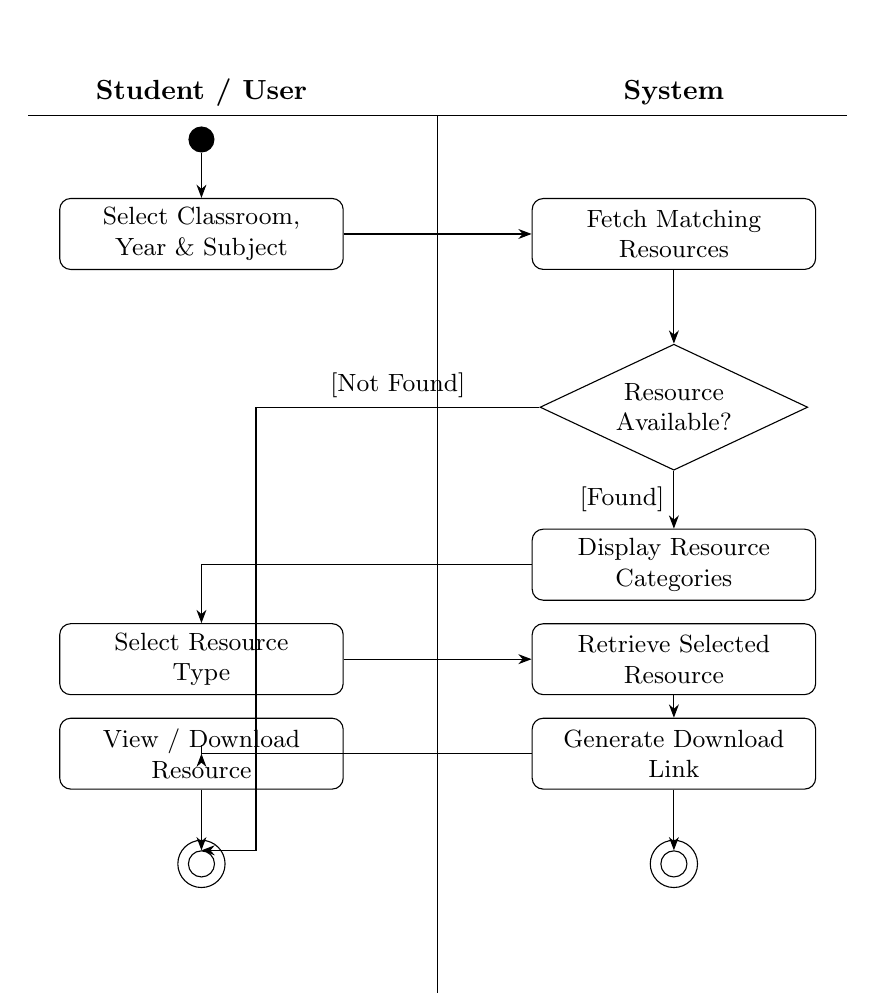
\begin{tikzpicture}[
        font=\small,
        box/.style={draw, rounded corners, minimum width=3.6cm, minimum height=0.9cm, align=center},
        dec/.style={draw, diamond, aspect=2, minimum width=3.4cm, minimum height=1.6cm, align=center, inner sep=1pt},
        >={Stealth[]}
      ]
        % lane headers and divider
        \node[font=\bfseries] at (0,0.6) {Student / User};
        \node[font=\bfseries] at (6,0.6) {System};
        \draw (3,0.3) -- (3,-11);
        \draw (-2.2,0.3) -- (8.2,0.3);

        \node[circle, fill=black, minimum size=0.25cm] (start) at (0,0) {};
        \node[box] (sel) at (0,-1.2) {Select Classroom,\\Year \& Subject};
        \node[box] (fetch) at (6,-1.2) {Fetch Matching\\Resources};
        \node[dec] (avail) at (6,-3.4) {Resource\\Available?};
        \node[box] (disp) at (6,-5.4) {Display Resource\\Categories};
        \node[box] (seltype) at (0,-6.6) {Select Resource\\Type};
        \node[box] (retrieve) at (6,-6.6) {Retrieve Selected\\Resource};
        \node[box] (link) at (6,-7.8) {Generate Download\\Link};
        \node[box] (view) at (0,-7.8) {View / Download\\Resource};
        \node[circle, draw, minimum size=0.22cm] (endL) at (0,-9.2) {};
        \draw (endL) circle (0.3cm);
        \node[circle, draw, minimum size=0.22cm] (endR) at (6,-9.2) {};
        \draw (endR) circle (0.3cm);

        \draw[->] (start) -- (sel);
        \draw[->] (sel) -- (fetch);
        \draw[->] (fetch) -- (avail);
        \draw[->] (avail) -- node[left]{[Found]} (disp);
        \draw[->] (avail.west) -- ++(-3.6,0) node[midway,above]{[Not Found]} |- (endL.north);
        \draw[->] (disp) -| (seltype);
        \draw[->] (seltype) -- (retrieve);
        \draw[->] (retrieve) -- (link);
        \draw[->] (link) -| (view);
        \draw[->] (view) -- (endL);
        \draw[->] (link) -- (endR);
    \end{tikzpicture}
    \caption{Swimlane Diagram -- Resource Access Flow}
\end{figure}

This diagram details the resource-access flow specifically: after the user selects a classroom,
year, and subject, the system fetches matching resources and checks whether a resource is
available. If not found, the flow ends; if found, the system displays resource categories, the user
selects a resource type, and the system retrieves the resource and generates a download link for
the user to view or download.

% --- Figure 2.4: Sequence Diagram ---
\begin{figure}[H]
    \centering
    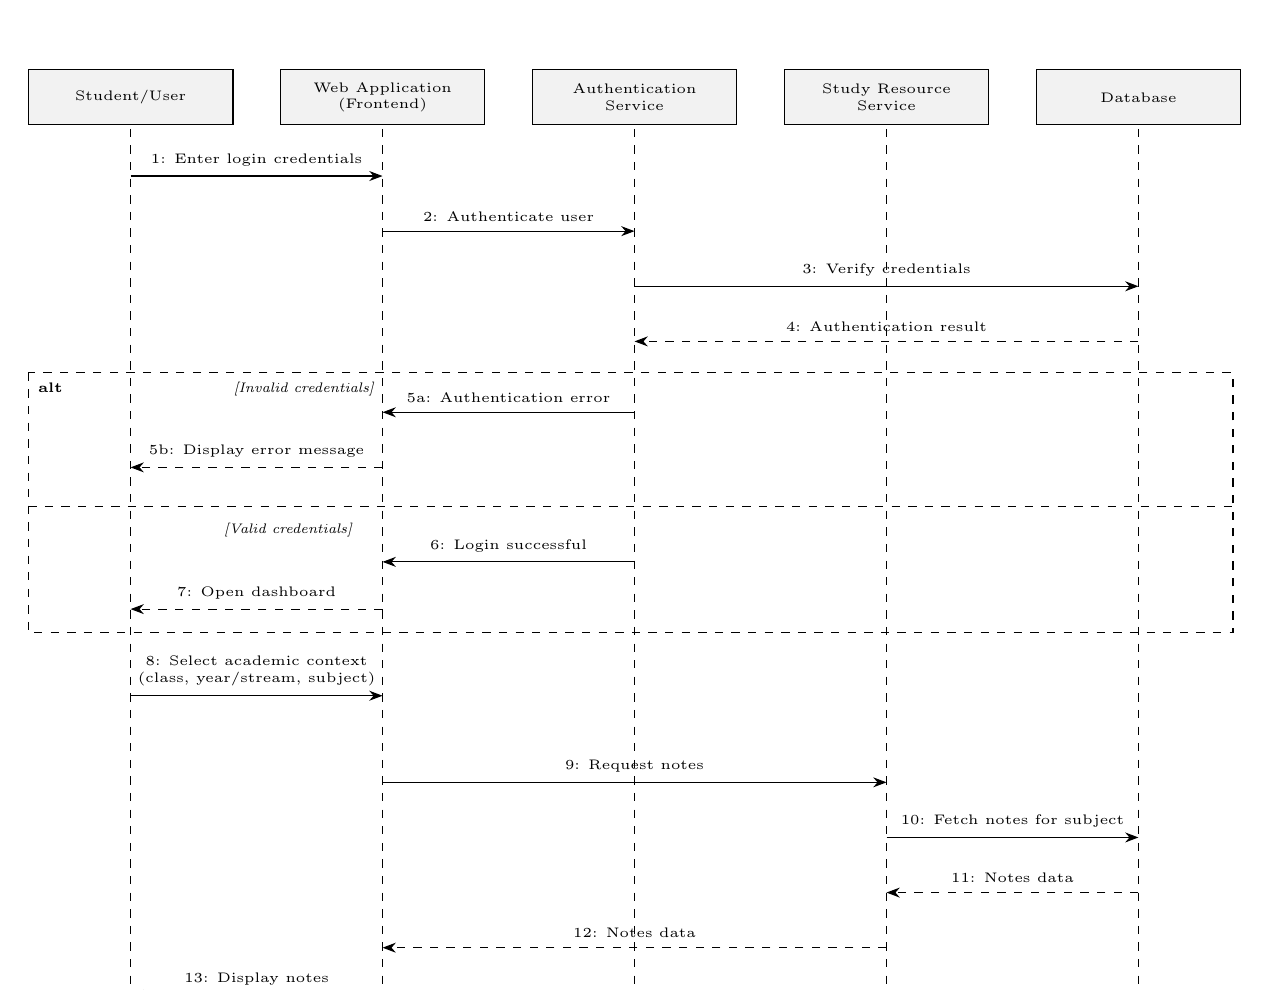
\begin{tikzpicture}[font=\tiny, >={Stealth[]}]
        \def\Ux{0} \def\Wx{3.2} \def\Ax{6.4} \def\Sx{9.6} \def\Dx{12.8}
        \node[draw, fill=gray!10, minimum width=2.6cm, minimum height=0.7cm, align=center] (U) at (\Ux,0) {Student/User};
        \node[draw, fill=gray!10, minimum width=2.6cm, minimum height=0.7cm, align=center] (W) at (\Wx,0) {Web Application\\(Frontend)};
        \node[draw, fill=gray!10, minimum width=2.6cm, minimum height=0.7cm, align=center] (A) at (\Ax,0) {Authentication\\Service};
        \node[draw, fill=gray!10, minimum width=2.6cm, minimum height=0.7cm, align=center] (S) at (\Sx,0) {Study Resource\\Service};
        \node[draw, fill=gray!10, minimum width=2.6cm, minimum height=0.7cm, align=center] (D) at (\Dx,0) {Database};

        \draw[dashed] (\Ux,-0.4) -- (\Ux,-11.5);
        \draw[dashed] (\Wx,-0.4) -- (\Wx,-11.5);
        \draw[dashed] (\Ax,-0.4) -- (\Ax,-11.5);
        \draw[dashed] (\Sx,-0.4) -- (\Sx,-11.5);
        \draw[dashed] (\Dx,-0.4) -- (\Dx,-11.5);

        \draw[->] (\Ux,-1.0) -- node[above]{1: Enter login credentials} (\Wx,-1.0);
        \draw[->] (\Wx,-1.7) -- node[above]{2: Authenticate user} (\Ax,-1.7);
        \draw[->] (\Ax,-2.4) -- node[above]{3: Verify credentials} (\Dx,-2.4);
        \draw[->, dashed] (\Dx,-3.1) -- node[above]{4: Authentication result} (\Ax,-3.1);

        \draw[draw, dashed] (-1.3,-3.5) rectangle (14,-6.8);
        \node[anchor=north west, font=\bfseries\tiny] at (-1.3,-3.5) {alt};

        \draw[->] (\Ax,-4.0) -- node[above]{5a: Authentication error} (\Wx,-4.0);
        \draw[->, dashed] (\Wx,-4.7) -- node[above]{5b: Display error message} (\Ux,-4.7);
        \node[font=\tiny\itshape] at (2.2,-3.7) {[Invalid credentials]};

        \draw[dashed] (-1.3,-5.2) -- (14,-5.2);
        \node[font=\tiny\itshape] at (2.0,-5.5) {[Valid credentials]};
        \draw[->] (\Ax,-5.9) -- node[above]{6: Login successful} (\Wx,-5.9);
        \draw[->, dashed] (\Wx,-6.5) -- node[above]{7: Open dashboard} (\Ux,-6.5);

        \draw[->] (\Ux,-7.6) -- node[above,align=center]{8: Select academic context\\(class, year/stream, subject)} (\Wx,-7.6);
        \draw[->] (\Wx,-8.7) -- node[above]{9: Request notes} (\Sx,-8.7);
        \draw[->] (\Sx,-9.4) -- node[above]{10: Fetch notes for subject} (\Dx,-9.4);
        \draw[->, dashed] (\Dx,-10.1) -- node[above]{11: Notes data} (\Sx,-10.1);
        \draw[->, dashed] (\Sx,-10.8) -- node[above]{12: Notes data} (\Wx,-10.8);
        \draw[->, dashed] (\Wx,-11.4) -- node[above]{13: Display notes} (\Ux,-11.4);
    \end{tikzpicture}
    \caption{Sequence Diagram -- Login and Notes Retrieval}
\end{figure}

The sequence diagram shows the message exchange between the Student/User, the Web
Application (Frontend), the Authentication Service, the Study Resource Service, and the
Database for the login flow (including the invalid- and valid-credentials alternatives) followed
by the notes-retrieval flow after academic context selection.

% --- Figure 2.5: Collaboration Diagram ---
\begin{figure}[H]
    \centering
    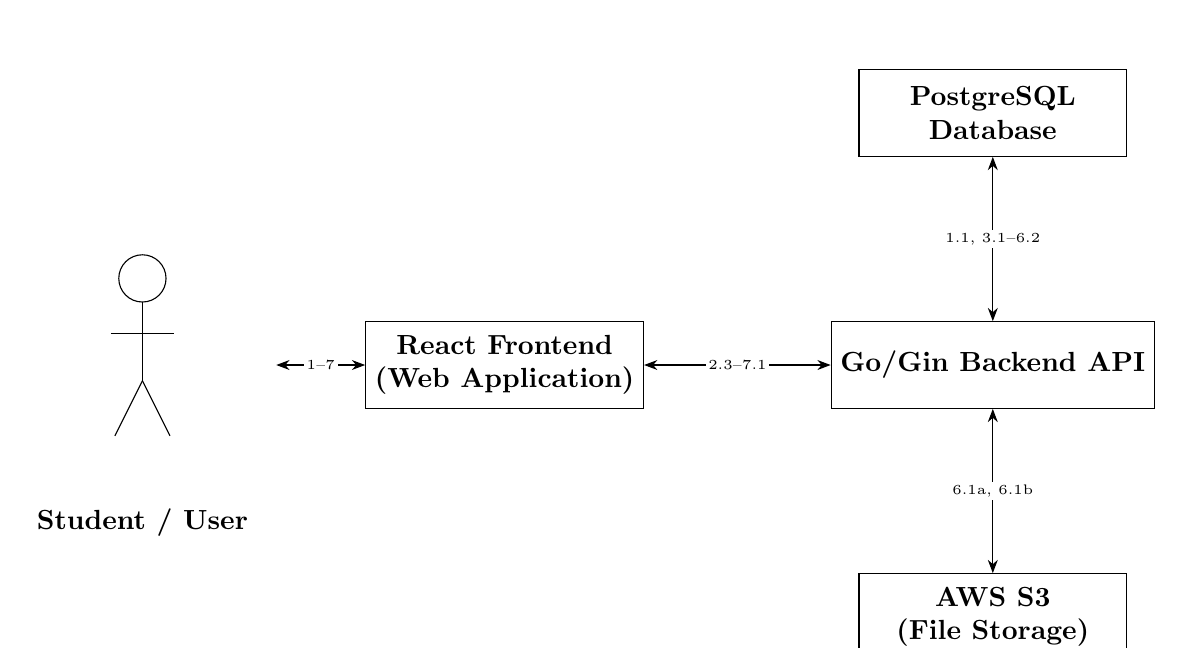
\begin{tikzpicture}[
        font=\small,
        obj/.style={draw, minimum width=3.4cm, minimum height=1.1cm, align=center, font=\bfseries},
        lbl/.style={font=\tiny, midway, fill=white, inner sep=1pt},
        >={Stealth[]}
      ]
        \begin{scope}[shift={(-4.6,-2.4)}]
            \draw (0,1.1) circle (0.3);
            \draw (0,0.8) -- (0,-0.2);
            \draw (-0.4,0.4) -- (0.4,0.4);
            \draw (0,-0.2) -- (-0.35,-0.9);
            \draw (0,-0.2) -- (0.35,-0.9);
            \node[font=\bfseries, yshift=-1.1cm] at (0,-0.9) {Student / User};
        \end{scope}
        \node[obj] (fe) at (0,-2.4)  {React Frontend\\(Web Application)};
        \node[obj] (be) at (6.2,-2.4)  {Go/Gin Backend API};
        \node[obj] (db) at (6.2,0.8) {PostgreSQL\\Database};
        \node[obj] (s3) at (6.2,-5.6) {AWS S3\\(File Storage)};

        \draw[<->] (-2.9,-2.4) -- node[lbl]{1--7} (fe);
        \draw[<->] (fe) -- node[lbl]{2.3--7.1} (be);
        \draw[<->] (be) -- node[lbl]{1.1, 3.1--6.2} (db);
        \draw[<->] (be) -- node[lbl]{6.1a, 6.1b} (s3);
    \end{tikzpicture}

    \vspace{0.4cm}
    \begin{center}
    \begin{minipage}{0.9\textwidth}
    \tiny
    \textbf{Message key:} \\
    1: enterCredentials() \quad
    2: selectAcademicContext() \quad
    2.1: selectYearAndStream() \quad
    2.2: selectSubject() \\
    3--5: request/send Notes, Books, PYQs \quad
    3.5/4.5/5.5: viewOrDownloadNotes/Books/PYQs() \\
    6: uploadStudyMaterial() \quad
    6.1: uploadStudyMaterial(metadata) \quad
    6.1a: uploadFile(file) \quad
    6.1b: fileUploadResult() \\
    6.2: storeMetadata() \quad
    6.3: uploadResponse() \quad
    6.4: uploadSuccess() \quad
    7: logout() \quad
    7.1: logoutResponse() / confirmLogout() \\
    1.1: authenticateUser() \quad
    1.1.1: verifyUser() \quad
    1.2: authenticationResponse() \quad
    1.2a: displayDashboard() \quad
    1.3: displayAuthenticationError()
    \end{minipage}
    \end{center}
    \caption{Collaboration Diagram -- Collaborative Study Platform}
\end{figure}

The collaboration diagram illustrates the same set of interactions as the sequence diagram from
an object-collaboration perspective, showing numbered messages exchanged between the
Student/User, the React Frontend, the Go/Gin Backend API, the PostgreSQL Database, and
AWS S3 for authentication, resource retrieval, study material upload, and logout.

\subsection{Technical Stack}
\begin{itemize}[leftmargin=*]
    \item Frontend: React, TypeScript / TSX, Axios, Tailwind CSS
    \item Backend: Go, Gin framework, REST-style APIs
    \item Database: PostgreSQL
    \item File Storage: AWS S3
\end{itemize}

\section{Implementation Details}

\subsection{Module 1: Core Functionality -- Authentication and Academic Navigation}
The authentication module allows a Student/User to Login or Register. The Frontend sends an
authentication request to the Backend, which verifies the user's credentials. If the credentials
are invalid, an authentication error is displayed and the user returns to the Login/Register
screen; if valid, the Dashboard is opened. After successful authentication, the user reaches the
Dashboard and selects their academic context in sequence: Classroom/Academic Context, then
Year/Stream, then Subject, before choosing a study action (View Notes, View/Download
Books, View/Download PYQs, or Upload Study Material).

\end{document}
